%%%% Paramétrage du cours %%%%
\def\xxactivite{Cours}
\def\xxauteur{\textsl{Xavier Pessoles}}

\fichefalse
\proftrue
\tdfalse
\courstrue

\def\xxnumchapitre{Chapitre 3 \vspace{.2cm}}
\def\xxchapitre{\hspace{.12cm} Application du Principe Fondamental de la Dynamique}

\def\xxcompetences{%
\textsl{%
\textbf{Savoirs et compétences :}\\
\begin{itemize}[label=\ding{112},font=\color{ocre}] 
\item \textit{Mod2.C16} : torseur cinétique
\item \textit{Mod2.C17} : torseur dynamique
\item \textit{Mod2.C17.SF1} : déterminer le torseur dynamique d’un solide, ou d’un ensemble de solides, par rapport à un autre solide
\item \textit{Mod2.C15} : matrice d'inertie
\item \textit{Res1.C2} : principe fondamental de la dynamique
\item \textit{Res1.C1.SF1} : proposer une démarche permettant la détermination de la loi de mouvement
\item \textit{Res1.C2.SF1} : proposer une méthode permettant la détermination d’une inconnue de liaison
\end{itemize}
}}
		
\def\xxfigures{
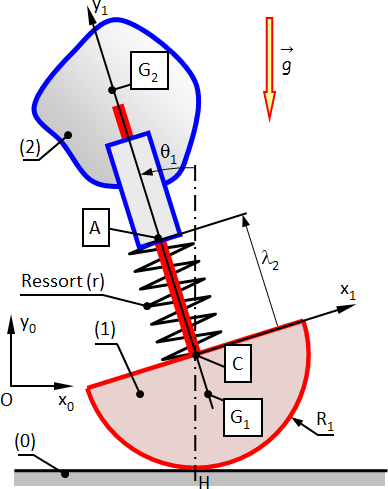
\includegraphics[width=4cm]{fig_01}\\
\textit{Toupie}

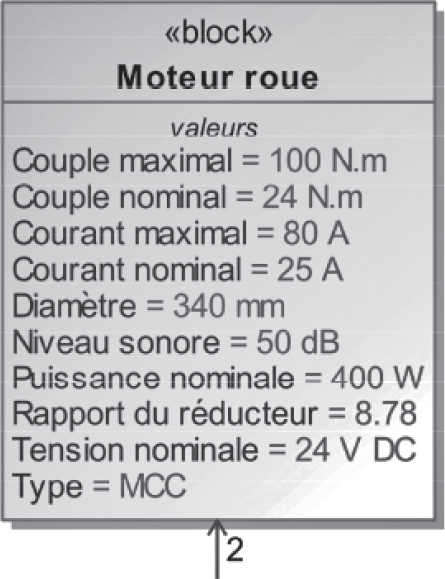
\includegraphics[width=4cm]{fig_02}\\
\textit{Volants d'inertie d'un vilebrequin}

}%figues de la page de garde


\iflivret
\pagestyle{empty}


%%%%%%%% PAGE DE GARDE COURS
\ifcours
% ==== BANDEAU DES TITRES ==== 
\begin{tikzpicture}[remember picture,overlay]
\node at (current page.north west)
{\begin{tikzpicture}[remember picture,overlay]
\node[anchor=north west,inner sep=0pt] at (0,0) {\includegraphics[width=\paperwidth]{\thechapterimage}};
\draw[anchor=west] (-2cm,-8cm) node [line width=2pt,rounded corners=15pt,draw=ocre,fill=white,fill opacity=0.6,inner sep=40pt]{\strut\makebox[22cm]{}};
\draw[anchor=west] (1cm,-8cm) node {\huge\sffamily\bfseries\color{black} %
\begin{minipage}{1cm}
\rotatebox{90}{\LARGE\sffamily\textsc{\color{ocre}\textbf{\xxnumpartie}}}
\end{minipage} \hfill
\begin{minipage}[c]{14cm}
\begin{titrepartie}
\begin{flushright}
\renewcommand{\baselinestretch}{1.1} 
\Large\sffamily\textsc{\textbf{\xxpartie}}
\renewcommand{\baselinestretch}{1} 
\end{flushright}
\end{titrepartie}
\end{minipage} \hfill
\begin{minipage}[c]{3.5cm}
{\large\sffamily\textsc{\textbf{\color{ocre} \discipline}}}
\end{minipage} 
 };
\end{tikzpicture}};
\end{tikzpicture}
% ==== FIN BANDEAU DES TITRES ==== 


% ==== ONGLET 
\begin{tikzpicture}[overlay]
\node[shape=rectangle, 
      rounded corners = .25 cm,
	  draw= ocre,
	  line width=2pt, 
	  fill = ocre!10,
	  minimum width  = 2.5cm,
	  minimum height = 3cm,] at (18.3cm,0) {};
\node at (17.7cm,0) {\rotatebox{90}{\textbf{\Large\color{ocre}{\classe}}}};
%{};
\end{tikzpicture}
% ==== FIN ONGLET 


\vspace{3.5cm}

\begin{tikzpicture}[remember picture,overlay]
\draw[anchor=west] (-2cm,-6cm) node {\huge\sffamily\bfseries\color{black} %
\begin{minipage}{2cm}
\begin{center}
\LARGE\sffamily\textsc{\color{ocre}\textbf{\xxactivite}}
\end{center}
\end{minipage} \hfill
\begin{minipage}[c]{15cm}
\begin{titrechapitre}
\renewcommand{\baselinestretch}{1.1} 
\Large\sffamily\textsc{\textbf{\xxnumchapitre}}

\Large\sffamily\textsc{\textbf{\xxchapitre}}
\vspace{.5cm}

\renewcommand{\baselinestretch}{1} 
\normalsize\normalfont
\xxcompetences
\end{titrechapitre}
\end{minipage}  };
\end{tikzpicture}
\vfill

\begin{flushright}
\begin{minipage}[c]{.3\linewidth}
\begin{center}
\xxfigures
\end{center}
\end{minipage}\hfill
\begin{minipage}[c]{.6\linewidth}
\startcontents
%\printcontents{}{1}{}
\printcontents{}{1}{}
\end{minipage}
\end{flushright}

\begin{tikzpicture}[remember picture,overlay]
\draw[anchor=west] (4.5cm,-.7cm) node {
\begin{minipage}[c]{.2\linewidth}
\begin{flushright}

\includegraphics[width=2cm]{logoCC}
\end{flushright}
\end{minipage}
\begin{minipage}[c]{.2\linewidth}
\textsl{\xxauteur} \\
\textsl{\classe}
\end{minipage}
 };
\end{tikzpicture}

\newpage
\pagestyle{fancy}

%\newpage
%\pagestyle{fancy}

\else
\fi
%% FIN PAGE DE GARDE DES COURS

%%%%%%%% PAGE DE GARDE TD
\iftd
%\begin{tikzpicture}[remember picture,overlay]
%\node at (current page.north west)
%{\begin{tikzpicture}[remember picture,overlay]
%\draw[anchor=west] (-2cm,-3.25cm) node [line width=2pt,rounded corners=15pt,draw=ocre,fill=white,fill opacity=0.6,inner sep=40pt]{\strut\makebox[22cm]{}};
%\draw[anchor=west] (1cm,-3.25cm) node {\huge\sffamily\bfseries\color{black} %
%\begin{minipage}{1cm}
%\rotatebox{90}{\LARGE\sffamily\textsc{\color{ocre}\textbf{\xxnumpartie}}}
%\end{minipage} \hfill
%\begin{minipage}[c]{13.5cm}
%\begin{titrepartie}
%\begin{flushright}
%\renewcommand{\baselinestretch}{1.1} 
%\Large\sffamily\textsc{\textbf{\xxpartie}}
%\renewcommand{\baselinestretch}{1} 
%\end{flushright}
%\end{titrepartie}
%\end{minipage} \hfill
%\begin{minipage}[c]{3.5cm}
%{\large\sffamily\textsc{\textbf{\color{ocre} \discipline}}}
%\end{minipage} 
% };
%\end{tikzpicture}};
%\end{tikzpicture}

%%%%%%%%%% PAGE DE GARDE TD %%%%%%%%%%%%%%%
%\begin{tikzpicture}[overlay]
%\node[shape=rectangle, 
%      rounded corners = .25 cm,
%	  draw= ocre,
%	  line width=2pt, 
%	  fill = ocre!10,
%	  minimum width  = 2.5cm,
%	  minimum height = 2.5cm,] at (18.5cm,0) {};
%\node at (17.7cm,0) {\rotatebox{90}{\textbf{\Large\color{ocre}{\classe}}}};
%%{};
%\end{tikzpicture}

% PARTIE ET CHAPITRE
%\begin{tikzpicture}[remember picture,overlay]
%\draw[anchor=west] (-1cm,-2.1cm) node {\large\sffamily\bfseries\color{black} %
%\begin{minipage}[c]{15cm}
%\begin{flushleft}
%\xxnumchapitre \\
%\xxchapitre
%\end{flushleft}
%\end{minipage}  };
%\end{tikzpicture}

% BANDEAU EXO
\iflivret % SI LIVRET
\begin{tikzpicture}[remember picture,overlay]
\draw[anchor=west] (-2cm,-3.3cm) node {\huge\sffamily\bfseries\color{black} %
\begin{minipage}{5cm}
\begin{center}
\LARGE\sffamily\color{ocre}\textbf{\textsc{\xxactivite}}

\begin{center}
\xxfigures
\end{center}

\end{center}
\end{minipage} \hfill
\begin{minipage}[c]{12cm}
\begin{titrechapitre}
\renewcommand{\baselinestretch}{1.1} 
\large\sffamily\textbf{\textsc{\xxtitreexo}}

\small\sffamily{\textbf{\textit{\color{black!70}\xxsourceexo}}}
\vspace{.5cm}

\renewcommand{\baselinestretch}{1} 
\normalsize\normalfont
\xxcompetences
\end{titrechapitre}
\end{minipage}};
\end{tikzpicture}
\else % ELSE NOT LIVRET
\begin{tikzpicture}[remember picture,overlay]
\draw[anchor=west] (-2cm,-4.5cm) node {\huge\sffamily\bfseries\color{black} %
\begin{minipage}{5cm}
\begin{center}
\LARGE\sffamily\color{ocre}\textbf{\textsc{\xxactivite}}

\begin{center}
\xxfigures
\end{center}

\end{center}
\end{minipage} \hfill
\begin{minipage}[c]{12cm}
\begin{titrechapitre}
\renewcommand{\baselinestretch}{1.1} 
\large\sffamily\textbf{\textsc{\xxtitreexo}}

\small\sffamily{\textbf{\textit{\color{black!70}\xxsourceexo}}}
\vspace{.5cm}

\renewcommand{\baselinestretch}{1} 
\normalsize\normalfont
\xxcompetences
\end{titrechapitre}
\end{minipage}};
\end{tikzpicture}

\fi

\else   % FIN IF TD
\fi


%%%%%%%% PAGE DE GARDE FICHE
\iffiche
\begin{tikzpicture}[remember picture,overlay]
\node at (current page.north west)
{\begin{tikzpicture}[remember picture,overlay]
\draw[anchor=west] (-2cm,-2.25cm) node [line width=2pt,rounded corners=15pt,draw=ocre,fill=white,fill opacity=0.6,inner sep=40pt]{\strut\makebox[22cm]{}};
\draw[anchor=west] (1cm,-2.25cm) node {\huge\sffamily\bfseries\color{black} %
\begin{minipage}{1cm}
\rotatebox{90}{\LARGE\sffamily\textsc{\color{ocre}\textbf{\xxnumpartie}}}
\end{minipage} \hfill
\begin{minipage}[c]{14cm}
\begin{titrepartie}
\begin{flushright}
\renewcommand{\baselinestretch}{1.1} 
\large\sffamily\textsc{\textbf{\xxpartie} \\} 

\vspace{.2cm}

\normalsize\sffamily\textsc{\textbf{\xxnumchapitre -- \xxchapitre}}
\renewcommand{\baselinestretch}{1} 
\end{flushright}
\end{titrepartie}
\end{minipage} \hfill
\begin{minipage}[c]{3.5cm}
{\large\sffamily\textsc{\textbf{\color{ocre} \discipline}}}
\end{minipage} 
 };
\end{tikzpicture}};
\end{tikzpicture}

\iflivret
\begin{tikzpicture}[overlay]
\node[shape=rectangle, 
      rounded corners = .25 cm,
	  draw= ocre,
	  line width=2pt, 
	  fill = ocre!10,
	  minimum width  = 2.5cm,
	  minimum height = 2.5cm,] at (18.5cm,.5cm) {};
\node at (17.9cm,.5cm) {\rotatebox{90}{\textsf{\textbf{\large\color{ocre}{\classe}}}}};
%{};
\end{tikzpicture}
\else
\begin{tikzpicture}[overlay]
\node[shape=rectangle, 
      rounded corners = .25 cm,
	  draw= ocre,
	  line width=2pt, 
	  fill = ocre!10,
	  minimum width  = 2.5cm,
%	  minimum height = 2.5cm,] at (18.5cm,1.1cm) {};
	  minimum height = 2.5cm,] at (18.6cm,0.5cm) {};
\node at (18cm,0.5cm) {\rotatebox{90}{\textsf{\textbf{\large\color{ocre}{\classe}}}}};
%{};
\end{tikzpicture}

\fi

\else
\fi



\else
\pagestyle{empty}


%%%%%%%% PAGE DE GARDE COURS
\ifcours
% ==== BANDEAU DES TITRES ==== 
\begin{tikzpicture}[remember picture,overlay]
\node at (current page.north west)
{\begin{tikzpicture}[remember picture,overlay]
\node[anchor=north west,inner sep=0pt] at (0,0) {\includegraphics[width=\paperwidth]{\thechapterimage}};
\draw[anchor=west] (-2cm,-8cm) node [line width=2pt,rounded corners=15pt,draw=ocre,fill=white,fill opacity=0.6,inner sep=40pt]{\strut\makebox[22cm]{}};
\draw[anchor=west] (1cm,-8cm) node {\huge\sffamily\bfseries\color{black} %
\begin{minipage}{1cm}
\rotatebox{90}{\LARGE\sffamily\textsc{\color{ocre}\textbf{\xxnumpartie}}}
\end{minipage} \hfill
\begin{minipage}[c]{14cm}
\begin{titrepartie}
\begin{flushright}
\renewcommand{\baselinestretch}{1.1} 
\Large\sffamily\textsc{\textbf{\xxpartie}}
\renewcommand{\baselinestretch}{1} 
\end{flushright}
\end{titrepartie}
\end{minipage} \hfill
\begin{minipage}[c]{3.5cm}
{\large\sffamily\textsc{\textbf{\color{ocre} \discipline}}}
\end{minipage} 
 };
\end{tikzpicture}};
\end{tikzpicture}
% ==== FIN BANDEAU DES TITRES ==== 


% ==== ONGLET 
\begin{tikzpicture}[overlay]
\node[shape=rectangle, 
      rounded corners = .25 cm,
	  draw= ocre,
	  line width=2pt, 
	  fill = ocre!10,
	  minimum width  = 2.5cm,
	  minimum height = 3cm,] at (18.3cm,0) {};
\node at (17.7cm,0) {\rotatebox{90}{\textbf{\Large\color{ocre}{\classe}}}};
%{};
\end{tikzpicture}
% ==== FIN ONGLET 


\vspace{3.5cm}

\begin{tikzpicture}[remember picture,overlay]
\draw[anchor=west] (-2cm,-6cm) node {\huge\sffamily\bfseries\color{black} %
\begin{minipage}{2cm}
\begin{center}
\LARGE\sffamily\textsc{\color{ocre}\textbf{\xxactivite}}
\end{center}
\end{minipage} \hfill
\begin{minipage}[c]{15cm}
\begin{titrechapitre}
\renewcommand{\baselinestretch}{1.1} 
\Large\sffamily\textsc{\textbf{\xxnumchapitre}}

\Large\sffamily\textsc{\textbf{\xxchapitre}}
\vspace{.5cm}

\renewcommand{\baselinestretch}{1} 
\normalsize\normalfont
\xxcompetences
\end{titrechapitre}
\end{minipage}  };
\end{tikzpicture}
\vfill

\begin{flushright}
\begin{minipage}[c]{.3\linewidth}
\begin{center}
\xxfigures
\end{center}
\end{minipage}\hfill
\begin{minipage}[c]{.6\linewidth}
\startcontents
%\printcontents{}{1}{}
\printcontents{}{1}{}
\end{minipage}
\end{flushright}

\begin{tikzpicture}[remember picture,overlay]
\draw[anchor=west] (4.5cm,-.7cm) node {
\begin{minipage}[c]{.2\linewidth}
\begin{flushright}

\includegraphics[width=2cm]{logoCC}
\end{flushright}
\end{minipage}
\begin{minipage}[c]{.2\linewidth}
\textsl{\xxauteur} \\
\textsl{\classe}
\end{minipage}
 };
\end{tikzpicture}

\newpage
\pagestyle{fancy}

%\newpage
%\pagestyle{fancy}

\else
\fi
%% FIN PAGE DE GARDE DES COURS

%%%%%%%% PAGE DE GARDE TD
\iftd
%\begin{tikzpicture}[remember picture,overlay]
%\node at (current page.north west)
%{\begin{tikzpicture}[remember picture,overlay]
%\draw[anchor=west] (-2cm,-3.25cm) node [line width=2pt,rounded corners=15pt,draw=ocre,fill=white,fill opacity=0.6,inner sep=40pt]{\strut\makebox[22cm]{}};
%\draw[anchor=west] (1cm,-3.25cm) node {\huge\sffamily\bfseries\color{black} %
%\begin{minipage}{1cm}
%\rotatebox{90}{\LARGE\sffamily\textsc{\color{ocre}\textbf{\xxnumpartie}}}
%\end{minipage} \hfill
%\begin{minipage}[c]{13.5cm}
%\begin{titrepartie}
%\begin{flushright}
%\renewcommand{\baselinestretch}{1.1} 
%\Large\sffamily\textsc{\textbf{\xxpartie}}
%\renewcommand{\baselinestretch}{1} 
%\end{flushright}
%\end{titrepartie}
%\end{minipage} \hfill
%\begin{minipage}[c]{3.5cm}
%{\large\sffamily\textsc{\textbf{\color{ocre} \discipline}}}
%\end{minipage} 
% };
%\end{tikzpicture}};
%\end{tikzpicture}

%%%%%%%%%% PAGE DE GARDE TD %%%%%%%%%%%%%%%
%\begin{tikzpicture}[overlay]
%\node[shape=rectangle, 
%      rounded corners = .25 cm,
%	  draw= ocre,
%	  line width=2pt, 
%	  fill = ocre!10,
%	  minimum width  = 2.5cm,
%	  minimum height = 2.5cm,] at (18.5cm,0) {};
%\node at (17.7cm,0) {\rotatebox{90}{\textbf{\Large\color{ocre}{\classe}}}};
%%{};
%\end{tikzpicture}

% PARTIE ET CHAPITRE
%\begin{tikzpicture}[remember picture,overlay]
%\draw[anchor=west] (-1cm,-2.1cm) node {\large\sffamily\bfseries\color{black} %
%\begin{minipage}[c]{15cm}
%\begin{flushleft}
%\xxnumchapitre \\
%\xxchapitre
%\end{flushleft}
%\end{minipage}  };
%\end{tikzpicture}

% BANDEAU EXO
\iflivret % SI LIVRET
\begin{tikzpicture}[remember picture,overlay]
\draw[anchor=west] (-2cm,-3.3cm) node {\huge\sffamily\bfseries\color{black} %
\begin{minipage}{5cm}
\begin{center}
\LARGE\sffamily\color{ocre}\textbf{\textsc{\xxactivite}}

\begin{center}
\xxfigures
\end{center}

\end{center}
\end{minipage} \hfill
\begin{minipage}[c]{12cm}
\begin{titrechapitre}
\renewcommand{\baselinestretch}{1.1} 
\large\sffamily\textbf{\textsc{\xxtitreexo}}

\small\sffamily{\textbf{\textit{\color{black!70}\xxsourceexo}}}
\vspace{.5cm}

\renewcommand{\baselinestretch}{1} 
\normalsize\normalfont
\xxcompetences
\end{titrechapitre}
\end{minipage}};
\end{tikzpicture}
\else % ELSE NOT LIVRET
\begin{tikzpicture}[remember picture,overlay]
\draw[anchor=west] (-2cm,-4.5cm) node {\huge\sffamily\bfseries\color{black} %
\begin{minipage}{5cm}
\begin{center}
\LARGE\sffamily\color{ocre}\textbf{\textsc{\xxactivite}}

\begin{center}
\xxfigures
\end{center}

\end{center}
\end{minipage} \hfill
\begin{minipage}[c]{12cm}
\begin{titrechapitre}
\renewcommand{\baselinestretch}{1.1} 
\large\sffamily\textbf{\textsc{\xxtitreexo}}

\small\sffamily{\textbf{\textit{\color{black!70}\xxsourceexo}}}
\vspace{.5cm}

\renewcommand{\baselinestretch}{1} 
\normalsize\normalfont
\xxcompetences
\end{titrechapitre}
\end{minipage}};
\end{tikzpicture}

\fi

\else   % FIN IF TD
\fi


%%%%%%%% PAGE DE GARDE FICHE
\iffiche
\begin{tikzpicture}[remember picture,overlay]
\node at (current page.north west)
{\begin{tikzpicture}[remember picture,overlay]
\draw[anchor=west] (-2cm,-2.25cm) node [line width=2pt,rounded corners=15pt,draw=ocre,fill=white,fill opacity=0.6,inner sep=40pt]{\strut\makebox[22cm]{}};
\draw[anchor=west] (1cm,-2.25cm) node {\huge\sffamily\bfseries\color{black} %
\begin{minipage}{1cm}
\rotatebox{90}{\LARGE\sffamily\textsc{\color{ocre}\textbf{\xxnumpartie}}}
\end{minipage} \hfill
\begin{minipage}[c]{14cm}
\begin{titrepartie}
\begin{flushright}
\renewcommand{\baselinestretch}{1.1} 
\large\sffamily\textsc{\textbf{\xxpartie} \\} 

\vspace{.2cm}

\normalsize\sffamily\textsc{\textbf{\xxnumchapitre -- \xxchapitre}}
\renewcommand{\baselinestretch}{1} 
\end{flushright}
\end{titrepartie}
\end{minipage} \hfill
\begin{minipage}[c]{3.5cm}
{\large\sffamily\textsc{\textbf{\color{ocre} \discipline}}}
\end{minipage} 
 };
\end{tikzpicture}};
\end{tikzpicture}

\iflivret
\begin{tikzpicture}[overlay]
\node[shape=rectangle, 
      rounded corners = .25 cm,
	  draw= ocre,
	  line width=2pt, 
	  fill = ocre!10,
	  minimum width  = 2.5cm,
	  minimum height = 2.5cm,] at (18.5cm,.5cm) {};
\node at (17.9cm,.5cm) {\rotatebox{90}{\textsf{\textbf{\large\color{ocre}{\classe}}}}};
%{};
\end{tikzpicture}
\else
\begin{tikzpicture}[overlay]
\node[shape=rectangle, 
      rounded corners = .25 cm,
	  draw= ocre,
	  line width=2pt, 
	  fill = ocre!10,
	  minimum width  = 2.5cm,
%	  minimum height = 2.5cm,] at (18.5cm,1.1cm) {};
	  minimum height = 2.5cm,] at (18.6cm,0.5cm) {};
\node at (18cm,0.5cm) {\rotatebox{90}{\textsf{\textbf{\large\color{ocre}{\classe}}}}};
%{};
\end{tikzpicture}

\fi

\else
\fi



\fi
\setlength{\columnseprule}{.1pt}

\vspace{2cm}
\pagestyle{fancy}
\thispagestyle{plain}



\section{Énoncé du Principe Fondamental de la Dynamique : cas général}

\begin{definition}[Énoncé du Principe Fondamental de la Dynamique]
Soit un ensemble matériel $E$ en mouvement par rapport à un référentiel galiléen ($R_0$), alors la somme des actions mécaniques extérieures s'appliquant sur $E$ est égale au torseur dynamique du mouvement de $E$ par rapport à $R_0$ :

$$
\torseurcin{D}{E}{R_0}=\torseurstat{T}{\overline{E}}{E}.
$$
De plus le \textbf{Principe Fondamental de la Dynamique} postule que pour tout mouvement, il existe au moins un référentiel dans lequel le PFD est vérifié. Ce sera donc un \textbf{référentiel galiléen}.


\begin{minipage}[c]{.48\linewidth}
Le \textbf{torseur dynamique} est de la forme : 
$$
\torseurcin{D}{E}{R_0}=\torseurl{
\vectrd{E}{R_0}=m\;\vectg{G}{E}{R_0}
}{
\vectmd{A}{E}{R_0}
}{A}.
$$

\end{minipage} \hfill
\begin{minipage}[c]{.48\linewidth}
\begin{itemize}
\item On note $\vectrd{S}{R_0}$ la résultante dynamique où l'accélération est \textbf{toujours} calculée au centre d'inertie $G$.
\item Le \textbf{moment dynamique} dépend du point A et se note $\vectmd{A}{E}{R_0}$.
\end{itemize}

\end{minipage} 

%\item On note $\overrightarrow{R_d}(E/R_0)$ la résultante du torseur dynamique : 
%
%$$\overrightarrow{R_d}(S/R_0)=m\;\overrightarrow{a}(G\in E/R_0)
%$$
%\item Le \textbf{moment dynamique} dépend du point A et se note $\vectmd{A}{E}{R_0}$
%\end{itemize}



\end{definition}


Du Principe Fondamental de la dynamique découle plusieurs \textbf{théorèmes généraux}.
\subsection{Théorème de la résultante dynamique}

		\begin{theorem}[Théorème de la résultante dynamique]
			Pour tout ensemble matériel $(E)$ de masse $m$ et de centre d'inertie $G$ en mouvement par rapport à un référentiel galiléen ($R_0$), la somme des résultantes des efforts extérieurs s'appliquant sur $E$ est égale à la résultante dynamique du mouvement de $E$ par rapport à $R_0$ :
$$
\vectf{\bar E}{E}=\vectrd{E}{R_0}=m\;\vectg{G}{E}{R_0}.
$$
	\end{theorem}


%\begin{rem}
%On peut alors définir un Newton comme l'effort à mettre en \oe{}uvre pour mettre en mouvement $\SI{1}{kg}$ avec une accélération de $\SI{1}{m.s^{-2}}$ en son centre de gravité $G$.
%\end{rem}

\subsection{Théorème du moment dynamique}
\begin{theorem}[Théorème du moment dynamique]
			Pour tout ensemble matériel $(E)$ de masse $m$ en mouvement par rapport à un référentiel galiléen ($R_0$), la somme des moments des efforts extérieurs s'appliquant sur $E$ en un point quelconque $A$ est égale au moment dynamique du mouvement de $E$ par rapport à $R_0$ en $A$ :
			$$
				\vectm{A}{\bar E}{E}=\vectmd{A}{E}{R_0}.
			$$
		\end{theorem}

%\begin{exemple}[Application à l'éolienne]
%\question{Déterminer le théorème à utiliser pour relier $C_m$ aux paramètres dynamique du problème.}
%
%\begin{texteCache}
%On pourra appliquer un théorème du moment dynamique s'appliquant sur l'éolienne ($E=\left\{1+2+3\right\}$) en projection sur l'axe $\couple{K}{\overrightarrow{z}_0}$  : 
%
%\begin{align*}
%\moment[K]{\bar E}{E}\cdot \overrightarrow{z}_0=\vDelta[K]{E}{R_0}\cdot \overrightarrow{z}_0.\\
%\\
%\Leftrightarrow\\
%C_m=\left(\vDelta[K]{1}{R_0}+\vDelta[K]{2}{R_0}+\vDelta[K]{3}{R_0}\right)\cdot \overrightarrow{z}_0
%\end{align*}
%\end{texteCache}
%
%\end{exemple}

\section{Torseur cinétique }

\subsection{Définition}
  \begin{definition}%[Torseur dynamique]
Le \textbf{torseur cinétique} d'un solide $S$ dans son mouvement par rapport à $R_0$ se définit de la façon suivante,

$$
\torseurcin{C}{S}{R_0}=\torseurl{\overrightarrow{R_c}(S/R_0)=\displaystyle{\int_{P\in S}}\overrightarrow{V}(P/R_0)\;\dd m}{\vectmc{A}{S}{R_0}=\displaystyle{\int_{P\in S}}\overrightarrow{AP}\wedge \overrightarrow{V}(P/R_0)\;\dd m}{A}
$$

\begin{itemize}
\item La résultante du torseur cinétique, $\overrightarrow{R_c}(S/R_0)$ ne dépend pas du point $A$ mais uniquement du centre de gravité $G$ de $S$ (de masse $m$) et vérifie :
$\overrightarrow{R_c}(S/R_0)=m\;\overrightarrow{V}(G/R_0).
$
\item Le moment cinétique dépend du point $A$ et peut s'exprimer avec la formule fondamentale de changement de point :
$
\vectmc{B}{S}{R_0}=\vectmc{A}{S}{R_0}+\overrightarrow{BA}\wedge \overrightarrow{R_c}(S/R_0).
$
\end{itemize}

\end{definition}


%\begin{demonstration}[Résultante cinétique]
%
%\begin{texteCache}
%\begin{align*}
%\overrightarrow{R_c}(S/R_0)=\displaystyle{\int_{P\in S}}\overrightarrow{V}(P/R_0)\;dm=
%\displaystyle{\int_{P\in S}}\left[\frac{d\overrightarrow{OP}}{\dd t}\right]_{R_0}\;dm\\
%=\displaystyle{\int_{P\in S}}\left[\frac{d(\overrightarrow{OG}+\overrightarrow{GP})}{\dd t}\right]_{R_0}\;dm
%=\displaystyle{\int_{P\in S}}\left[\frac{d\overrightarrow{OG}}{\dd t}\right]_{R_0}\;dm+\displaystyle{\int_{P\in S}}\left[\frac{d\overrightarrow{GP}}{\dd t}\right]_{R_0}\;dm.
%\end{align*}
%
%Or, $S$ est à masse conservative,
%
%\begin{align*}
%\displaystyle{\int_{P\in S}}\left[\frac{d\overrightarrow{GP}}{\dd t}\right]_{R_0}\;dm
%=\left[\frac{d}{\dd t}\left(\displaystyle{\int_{P\in S}}\overrightarrow{GP}\;dm\right)\right]_{R_0}=\overrightarrow{0}.
%\end{align*}
%
%On obtient alors,
%
%\begin{align*}
%\overrightarrow{R_c}(S/R_0)=\displaystyle{\int_{P\in S}}\left[\frac{d\overrightarrow{OG}}{\dd t}\right]_{R_0}\;dm
%=\left[\frac{d\overrightarrow{OG}}{\dd t}\right]_{R_0}\displaystyle{\int_{P\in S}}dm\\
%=m\;\overrightarrow{V}(G/R_0)\\
%\end{align*}
%
%\end{texteCache}
%\end{demonstration}

\subsection{Écriture avec l'opérateur d'inertie}

\begin{prop}
Pour un solide $S$ de masse $m$ dans son mouvement par rapport au repère $R_0$ et soit un point $A$ quelconque.
$$\vectmc{A}{S}{R_0}=\inertie{A}{S}\cdot \vecto{S}{R_0}+m\;\vect{AG}\wedge \vectv{A}{S}{R_0}.
$$
%\item \textbf{Dans la pratique}, il faudra utiliser cette formule.
%\end{itemize}
\end{prop}


%\begin{demonstration}
%\begin{texteCache}
%\begin{align*}
%\vSigma[A]{S}{R_0}=\displaystyle{\int_{P\in S}}\overrightarrow{AP}\wedge \overrightarrow{V}(P/R_0)\;dm
%=\displaystyle{\int_{P\in S}}\overrightarrow{AP}\wedge \overrightarrow{V}(P\in S/R_0)\;dm\\
%=\displaystyle{\int_{P\in S}}\overrightarrow{AP}\wedge \left(\overrightarrow{V}(A\in S/R_0)+\overrightarrow{\Omega}(S/R_0)\wedge \overrightarrow{AP}\right)\;dm\\
%=\overline{\overline{I}}_A(S)\cdot \overrightarrow{\Omega}(S/R_0)+M\;\overrightarrow{AG}\wedge \overrightarrow{V}(A\in S/R_0).
%\end{align*}
%\end{texteCache}
%\end{demonstration}

\subsection{Cas particuliers}

\begin{itemize}
\item En appliquant cette formule en un point \textbf{$A$ fixe} dans le mouvement de $S/R_0$, on a :$\vectmc{A}{S}{R_0}=\inertie{A}{S}\cdot \vecto{S}{R_0}$.
\item En appliquant cette formule en \textbf{$G$, centre d'inertie} de $S$, on a :
$
\vectmc{G}{S}{R_0}=\inertie{G}{S}\cdot \vecto{S}{R_0}.
$
\end{itemize}



\subsection{Méthodologie de Calcul}

On considère un ensemble matériel $E$ composé de solides $S_i$. On étudie son mouvement dans le référentiel $R_0$.
On donne la méthodologie de calcul du moment cinétique en un point $A$ sur la figure suivante.%\ref{algo_moment_cine}.

%\begin{figure}[htb]
\begin{center}
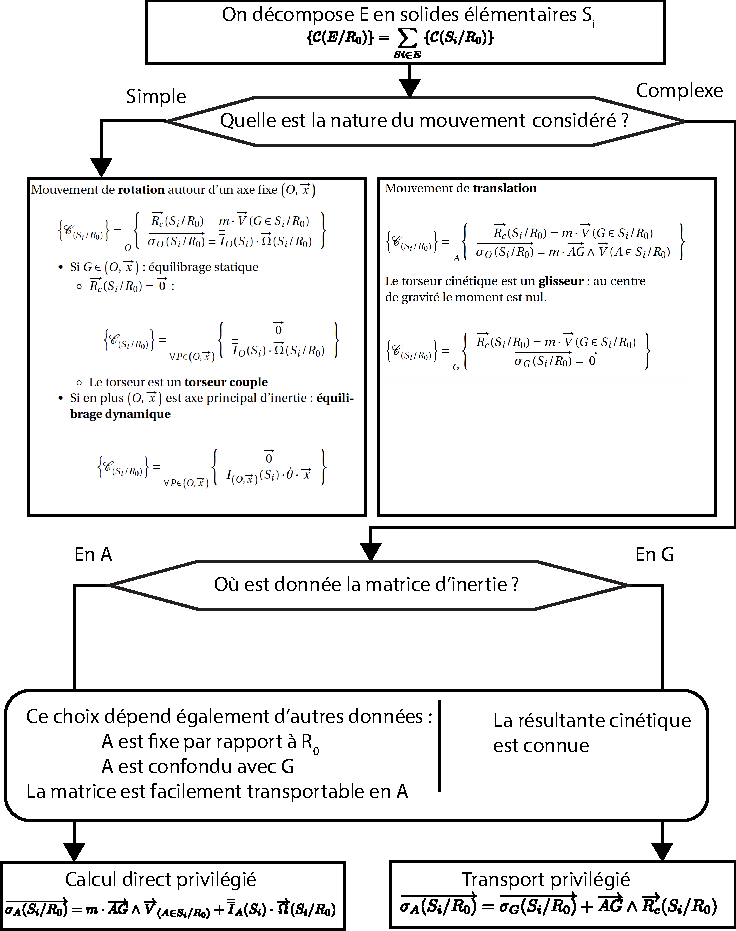
\includegraphics[width=.9\textwidth]{algorigramme_moment_cinetique.pdf}
%\caption{Algorigramme de calcul du moment cinétique \label{algo_moment_cine}}
\end{center}
%\end{figure}

%\begin{exemple}[Application à l'éolienne]
%\question{Déterminer la composante suivant $\overrightarrow{z}_0$ du moment cinétique au point K de la girouette 1 dans son mouvement par rapport au support 0, notée $\overrightarrow{z}_0\cdot \vectmc{K}{1}{0}$.}
%
%\begin{texteCache}
%\begin{itemize}
%\item Le mouvement de $1/0$ est un mouvement de rotation autour d'un axe fixe \couple{K}{\overrightarrow{z}_0} : 
%
%\item $\vectmc{K}{1}{0}\cdot \overrightarrow{z}_0=\left(\overline{\overline{I}}_K(1)\cdot \overrightarrow{\Omega}(1/0)\right)\cdot \overrightarrow{z}_0=\left(\overline{\overline{I}}_K(1)\cdot \dot{\alpha}\cdot \overrightarrow{z}_0 \right)\cdot \overrightarrow{z}_0$
%
%\item or on note J son moment d'inertie par rapport à l'axe \couple{K}{\overrightarrow{z}} soit : 
%\begin{align*}
%\overline{\overline{I}}_K(1)\cdot\overrightarrow{z}_0\cdot \overrightarrow{z}_0=J
%\end{align*}
%
%\item Ainsi : 
%
%\begin{align*}
%\boxed{
%\vectmc{K}{1}{0}\cdot \overrightarrow{z}_0=J\cdot \dot{\alpha}
%}
%\end{align*}
%\end{itemize}
%\end{texteCache}
%
%\question{Déterminer le moment cinétique $\vSigma[K]{2}{0}$  calculé au point K de l'hélice 2 dans son mouvement par rapport à 0.}
%
%\begin{texteCache}
%\begin{itemize}
%\item Le mouvement de $2/0$ n'est pas un mouvement simple. 
%\item On connaît l'opérateur d'inertie en G, on calcule donc : $\vSigma[G]{2}{0}$,
%
%\begin{align*}
%\vSigma[G]{2}{0}=\overline{\overline{I}}_G(2)\cdot \overrightarrow{\Omega}(2/0).
%\end{align*}
%
%\item On calcule $\overrightarrow{\Omega}(2/0)$
%\begin{align*}
%\overrightarrow{\Omega}(2/0)=\overrightarrow{\Omega}(2/1)+\overrightarrow{\Omega}(1/0)=
%\dot{\beta}\cdot \overrightarrow{x}_{1,2}+\dot{\alpha}\cdot \overrightarrow{z}_{1}
%\\=\dot{\beta}\cdot \overrightarrow{x}_{1,2}
%+\dot{\alpha}\left(\cos\beta\overrightarrow{z}_2+\sin\beta\overrightarrow{y}_2\right)\\
%\end{align*}
%
%\item On calcule $\vSigma[G]{2}{0}$ : 
%
%\begin{align*}
%\vSigma[G]{2}{0}=\left(
%\begin{array}{ccc}
%A & 0 & 0 \\ 
%0 & B & 0 \\ 
%0 & 0 & C
%\end{array}
%\right)_{\triplet{\overrightarrow{x}_2}{\overrightarrow{y}_2}{\overrightarrow{z}_2}} \cdot 
%\left(
%\begin{array}{c}
%\dot{\beta}\\
%\dot{\alpha}\cdot \sin\beta\\
%\dot{\alpha}\cdot \cos\beta\\
%\end{array}
%\right)_{\triplet{\overrightarrow{x}_2}{\overrightarrow{y}_2}{\overrightarrow{z}_2}}\\
%=\left(
%\begin{array}{c}
%A\cdot \dot{\beta}\\
%B\cdot \dot{\alpha}\cdot \sin\beta\\
%C\cdot \dot{\alpha}\cdot \cos\beta\\
%\end{array}
%\right)_{\triplet{\overrightarrow{x}_2}{\overrightarrow{y}_2}{\overrightarrow{z}_2}}\\
%\end{align*}
%\end{itemize}
%\end{texteCache}
%\end{exemple}

%\setcounter{cptExemple}{2}
%\begin{exemple}[Application à l'éolienne]
%\begin{texteCache}
%\begin{itemize}
%\item On calcule $\vSigma[K]{2}{0}$ : 
%
%\begin{itemize}
%\item \begin{align*}
%\vSigma[K]{2}{0}=\vSigma[G]{2}{0}+\overrightarrow{KG}\wedge \overrightarrow{R_c}(2/0)
%=\vSigma[G]{2}{0}+a\cdot \overrightarrow{x}_1\wedge M\cdot \overrightarrow{V}(G\in 2/0)
%\end{align*}
%
%\item On calcule $\overrightarrow{V}(G\in 2/0)$ : 
%
%\begin{align*}
%\overrightarrow{V}(G\in 2/0)=\overrightarrow{V}(K\in 2/0)+\overrightarrow{GK}\wedge \overrightarrow{\Omega}(2/0)=
%\overrightarrow{0}-a\cdot \overrightarrow{x}_1\wedge \left(\dot{\beta}\cdot \overrightarrow{x}_{1,2}+\dot{\alpha}\cdot \overrightarrow{z}_{1}\right)\\
%=a\cdot \dot{\alpha}\overrightarrow{y}_{1} 
%\end{align*}
%
%\item On calcule $a\cdot \overrightarrow{x}_1\wedge M\cdot \overrightarrow{V}(G\in 2/0)$ : 
%
%\begin{align*}
%a\cdot \overrightarrow{x}_1\wedge M\cdot \overrightarrow{V}(G\in 2/0)=
%a\cdot \overrightarrow{x}_1\wedge M\left(a\cdot \dot{\alpha}\overrightarrow{y}_{1} \right)=\\
%M\cdot a^2\cdot \dot{\alpha}\cdot \overrightarrow{z}_1
%\end{align*}
%
%\item On en déduit $\vSigma[K]{2}{0}$: 
%
%\begin{align*}
%\vSigma[K]{2}{0}=\left(
%\begin{array}{c}
%A\cdot \dot{\beta}\\
%B\cdot \dot{\alpha}\cdot \sin\beta+M\cdot a^2\cdot \dot{\alpha}\sin\beta\\
%C\cdot \dot{\alpha}\cdot \cos\beta+M\cdot a^2\cdot \dot{\alpha}\cos\beta\\
%\end{array}
%\right)_{\triplet{\overrightarrow{x}_2}{\overrightarrow{y}_2}{\overrightarrow{z}_2}}\\
%\end{align*}
%
%\end{itemize}
%
%\end{itemize}
%\end{texteCache}
%
%\question{Déterminer le moment cinétique $\vSigma[K]{3}{0}$.}
%
%\begin{texteCache}
%\begin{itemize}
%\item Le solide $3$ est solide à masse ponctuelle, ainsi $\vSigma[Q]{3}{0}=\overrightarrow{0}$.
%\item $\vSigma[K]{3}{0}=\overrightarrow{KQ}\wedge m\cdot \overrightarrow{V}(Q\in 3/0)$ : 
%\begin{itemize}
%\item On calcule $\overrightarrow{KQ}$ : 
%\begin{align*}
%\overrightarrow{KQ}=\overrightarrow{KG}+\overrightarrow{GQ}=a\cdot \overrightarrow{x}_1-b\cdot \overrightarrow{z}_2
%\end{align*}
%\item On calcule $\overrightarrow{V}(Q\in 3/0)$ : 
%
%\begin{align*}
%\overrightarrow{V}(Q\in 3/0)=\overrightarrow{V}(Q\in 3/2)+\overrightarrow{V}(Q\in 2/1)+\overrightarrow{V}(Q\in 1/0)
%\\
%=\overrightarrow{0}+\overrightarrow{V}(G\in 2/1)+\overrightarrow{QG}\wedge \overrightarrow{\Omega}(2/1)
%+\overrightarrow{V}(G\in 1/0)+\overrightarrow{QG}\wedge \overrightarrow{\Omega}(1/0)\\
%=\overrightarrow{0}+b\cdot \overrightarrow{z}_2\wedge \dot{\beta}\cdot \overrightarrow{x}_2+ a\cdot \dot{\alpha}\cdot \overrightarrow{y}_1+b\cdot \overrightarrow{z}_2\wedge \dot{\alpha}\cdot \overrightarrow{z}_1\\
%=b\cdot \dot{\beta}\cdot \overrightarrow{y}_2+a\cdot \dot{\alpha}\cdot \overrightarrow{y}_1-b\cdot\dot{\alpha} \sin\beta\cdot \overrightarrow{x}_{1,2}
%\end{align*}
%
%\item On calcule $\overrightarrow{KQ}\wedge m\overrightarrow{V}(Q\in 3/0)$ : 
%
%\begin{align*}
%\overrightarrow{KQ}\wedge m\overrightarrow{V}(Q\in 3/0)=m\cdot \left[a\cdot \overrightarrow{x}_1-b\cdot \overrightarrow{z}_2\right]\wedge\left[b\cdot \dot{\beta}\cdot \overrightarrow{y}_2+a\cdot \dot{\alpha}\cdot \overrightarrow{y}_1-b\cdot\dot{\alpha} \sin\beta\cdot \overrightarrow{x}_{1,2}\right]\\
%=m\left[a\cdot b\cdot \overrightarrow{z}_2+a^2\cdot \dot{\alpha}\cdot\overrightarrow{z}_1+b^2\cdot \dot{\beta}\cdot\overrightarrow{x}_2+b\cdot a\cdot \dot{\alpha}\cdot \cos\beta\cdot \overrightarrow{x}_1+b^2\cdot \dot{\alpha}\sin\beta\cdot \overrightarrow{y}_2\right]
%\end{align*}
%\end{itemize}
%
%\item,
%
%\begin{align*}
%\boxed{
%\vSigma[K]{3}{0}=m\left[a\cdot b\cdot\dot{\beta} \overrightarrow{z}_2+a^2\cdot \dot{\alpha}\cdot\overrightarrow{z}_1+b^2\cdot \dot{\beta}\cdot\overrightarrow{x}_2+b\cdot a\cdot \dot{\alpha}\cdot \cos\beta\cdot \overrightarrow{x}_1+b^2\cdot \dot{\alpha}\sin\beta\cdot \overrightarrow{y}_2\right]
%}
%\end{align*}
%\end{itemize}
%
%\end{texteCache}
%\end{exemple}


\section{Torseur dynamique}
\subsection{Définition}
\begin{definition}%[Torseur dynamique]
Le \textbf{torseur dynamique} d'un solide $S$ dans son mouvement par rapport à $R_0$ se définit de la façon suivante,

$$
\torseurcin{D}{S}{R_0}=\torseurl{\overrightarrow{R_d}(S/R_0)=\displaystyle{\int_{P\in S}}\overrightarrow{\Gamma}(P/R_0)\;\dd m}{\vectmd{A}{S}{R_0}=\displaystyle{\int_{P\in S}}\overrightarrow{AP}\wedge \overrightarrow{\Gamma}(P/R_0)\;\dd m}{A}
$$

\begin{itemize}
\item La résultante du torseur dynamique, $\overrightarrow{R_d}(S/R_0)$ ne dépend pas du point $A$ mais uniquement du centre de gravité $G$ de $S$ (de masse $m$) et vérifie : $\overrightarrow{R_d}(S/R_0)=m\;\overrightarrow{\Gamma}(G/R_0).$
\item Le moment dynamique dépend du point A et peut s'exprimer avec la formule fondamentale de changement de point :$
\vectmd{B}{S}{R_0}=\vectmd{A}{S}{R_0}+\overrightarrow{BA}\wedge \overrightarrow{R_d}(S/R_0).$
\end{itemize}

\end{definition}


%\begin{demonstration}[Résultante dynamique]

%\begin{texteCache}
%\begin{align*}
%\overrightarrow{R_d}(S/R_0)=\displaystyle{\int_{P\in S}}\overrightarrow{a}(P/R_0)\;dm=
%\displaystyle{\int_{P\in S}}\left[\frac{d^2\overrightarrow{OP}}{dt^2}\right]_{R_0}\;dm\\
%=\displaystyle{\int_{P\in S}}\left[\frac{d^2(\overrightarrow{OG}+\overrightarrow{GP})}{dt^2}\right]_{R_0}\;dm
%=\displaystyle{\int_{P\in S}}\left[\frac{d^2\overrightarrow{OG}}{dt^2}\right]_{R_0}\;dm+\displaystyle{\int_{P\in S}}\left[\frac{d^2\overrightarrow{GP}}{dt^2}\right]_{R_0}\;dm.
%\end{align*}
%
%Or, $S$ est à masse conservative,
%
%\begin{align*}
%\displaystyle{\int_{P\in S}}\left[\frac{d^2\overrightarrow{GP}}{dt^2}\right]_{R_0}\;dm
%=\left[\frac{d^2}{dt^2}\left(\displaystyle{\int_{P\in S}}\overrightarrow{GP}\;dm\right)\right]_{R_0}=\overrightarrow{0}.
%\end{align*}
%
%On obtient alors,
%
%\begin{align*}
%\overrightarrow{R_d}(S/R_0)=\displaystyle{\int_{P\in S}}\left[\frac{d^2\overrightarrow{OG}}{dt^2}\right]_{R_0}\;dm
%=\left[\frac{d^2\overrightarrow{OG}}{dt^2}\right]_{R_0}\displaystyle{\int_{P\in S}}dm\\
%=m\;\overrightarrow{a}(G/R_0)\\
%\end{align*}
%
%\end{texteCache}
%\end{demonstration}

\subsection{Relations entre les torseurs cinétiques et dynamiques}
\begin{prop}[Relations entre les torseurs cinétiques et dynamiques]
Pour un solide S de masse $M$ dans son mouvement par rapport au repère $R_0$ et soit un point $A$ quelconque.
\begin{itemize}
\item Relation entre les \textbf{résultantes} :$
\overrightarrow{R_d}(S/R_0)=\left[\frac{\dd \overrightarrow{R_c}(S/R_0)}{\dd t}\right]_{R_0}.$
\item Relation entre les \textbf{moments} :
$\vectmd{A}{S}{R_0}=\left[\frac{\dd \vectmc{A}{S}{R_0}}{\dd t}\right]_{R_0}+\overrightarrow{V(A/R_0)}\wedge \overrightarrow{R_c}(S/R_0).$
\end{itemize}
\end{prop}




\subsection{Cas particuliers}

%\begin{rem}
\begin{itemize}
\item En appliquant cette formule en un point \textbf{$O$ fixe} dans $R_0$, on a :
$\vectmd{O}{S}{R_0}=\left[\frac{\dd \vectmc{O}{S}{R_0}}{\dd t}\right]_{R_0}.$
\item En appliquant cette formule en un point \textbf{$G$, centre d'inertie de $S$}, on a :
$\vectmd{G}{S}{R_0}=\left[\frac{\dd \vectmc{G}{S}{R_0}}{\dd t}\right]_{R_0}.$
\end{itemize}
%\end{rem}





\newpage
\subsection{Méthodologie de calcul}

On considère un ensemble matériel $E$ composé de solides $S_i$. On étudie son mouvement dans le référentiel $R_0$.
On donne l'algorigramme de calcul du moment dynamique en un point $A$ sur la figure ci-dessous.%\ref{algo_moment_dyna}.

%\begin{exemple}[Application à l'éolienne]
%\question{Déterminer la composante suivant $\overrightarrow{z}_0$ du moment dynamique au point K de la girouette 1 dans son mouvement par rapport au support 0, notée $\overrightarrow{z}_0\cdot \vDelta[K]{1}{0}$.}
%
%\begin{texteCache}
%\begin{align*}
%\overrightarrow{z}_0\cdot \vDelta[K]{1}{0}=\overrightarrow{z}_0\cdot\left[\frac{d\vSigma[K]{1}{0}}{\dd t}\right]_{R_0}
%=\left[\frac{d\overrightarrow{z}_0\cdot\vSigma[K]{1}{0}}{\dd t}\right]_{R_0}=J\cdot \ddot{\alpha}
%\end{align*}
%\end{texteCache}
%
%\question{Déterminer la composante suivant $\overrightarrow{z}_0$ du moment dynamique $\overrightarrow{z}_0\cdot \vDelta[K]{2}{0}$.}
%
%\begin{texteCache}
%\begin{align*}
%\overrightarrow{z}_0\cdot \vDelta[K]{2}{0}=\overrightarrow{z}_0\cdot\left[\frac{d\vSigma[K]{2}{0}}{\dd t}\right]_{R_0}
%=\left[\frac{d\overrightarrow{z}_0\cdot\vSigma[K]{2}{0}}{\dd t}\right]_{R_0}
%\end{align*}
%
%Or, $\overrightarrow{z}_{0,1}=\cos\beta\cdot \overrightarrow{z}_2+\sin\beta\cdot \overrightarrow{y}_2$,
%
%\begin{align*}
%\overrightarrow{z}_0\cdot\vSigma[K]{2}{0}=
%\left(
%\begin{array}{c}
%A\cdot \dot{\beta}\\
%B\cdot \dot{\alpha}\cdot \sin\beta+M\cdot a^2\cdot \dot{\alpha}\sin\beta\\
%C\cdot \dot{\alpha}\cdot \cos\beta+M\cdot a^2\cdot \dot{\alpha}\cos\beta\\
%\end{array}
%\right)_{\triplet{\overrightarrow{x}_2}{\overrightarrow{y}_2}{\overrightarrow{z}_2}}
%\cdot
%\left(
%\begin{array}{c}
%0\\
%\sin\beta\\
%\cos\beta\\
%\end{array}
%\right)_{\triplet{\overrightarrow{x}_2}{\overrightarrow{y}_2}{\overrightarrow{z}_2}}
%\\
%=\dot{\alpha}\left[B\cdot \sin^2\beta+C\cdot \cos^2\beta+M\cdot a^2\right]
%\end{align*}
%
%d'où,
%\begin{align*}
%\boxed{
%\overrightarrow{z}_0\cdot \vDelta[K]{2}{0}=\ddot{\alpha}\left[B\cdot \sin^2\beta+C\cdot \cos^2\beta+M\cdot a^2\right]
%+2\cdot\dot{\alpha}\dot{\beta}\cdot \cos\beta\cdot \sin\beta\left[B-C\right].
%}
%\end{align*}
%
%\end{texteCache}
%
%\question{Déterminer la projection du moment dynamique de $3/0$ selon $\overrightarrow{z}_0$ : $\overrightarrow{z}_0\cdot \vSigma[K]{3}{0}$.}
%
%
%
%\begin{texteCache}
%\begin{minipage}{0.5\textwidth}
%\begin{center}
%\scFigCalc[x_{1,2}]{y_1}{z_1}{y_2}{z_2}{\beta}
%\end{center}
%\end{minipage}
%\begin{minipage}{0.5\textwidth}
%\begin{align*}
%\overrightarrow{z}_{0,1}\cdot \overrightarrow{z}_2=\cos\beta\\
%\overrightarrow{z}_{0,1}\cdot \overrightarrow{z}_1=1\\
%\overrightarrow{z}_{0,1}\cdot \overrightarrow{x}_0=0\\
%\overrightarrow{z}_{0,1}\cdot \overrightarrow{x}_1=0\\
%\overrightarrow{z}_1\cdot \overrightarrow{y}_2=\sin\beta\\
%\end{align*}
%\end{minipage}
%
%On trouve alors : 
%
%\begin{align*}
%\overrightarrow{z}_0\cdot \vSigma[K]{3}{0}=
%m\frac{d\left[a\cdot b\cdot \dot{\beta}\cos\beta+a^2\cdot \dot{\alpha}+b^2\cdot \dot{\alpha}\sin^2\beta\right]}{\dd t}\\
%=m\left[a\cdot b\cdot \left(\ddot{\beta}\cos\beta-\dot{\beta}^2\sin\beta\right)+a^2\ddot{\alpha}+b^2\cdot\left(\ddot{\alpha}\sin^2\beta+2\dot{\alpha}\dot{\beta}\sin\beta\cos\beta\right)\right]
%\end{align*}
%
%\end{texteCache}
%
%\question{Dans le cas d'une vitesse de rotation de l'hélice 2 ($\dot{\beta}$) constante et dans le cas où l'angle $\alpha$ est constant (pas de changement d'orientation de l'éolienne) déterminer l'expriment du couple $C_m$ que devrait fournir un moteur placé dans le mat (entre 0 et 1) pour "contrer" les effets dynamiques du balourd.}
%
%\begin{texteCache}
%Le théorème du moment dynamique autour de l'axe $\couple{K}{\overrightarrow{z}_{0,1}}$ donne :
%
%\begin{align*}
%C_m=-m\cdot a\cdot b\cdot \dot{\beta}^2\sin\beta
%\end{align*} 
%
%
%\end{texteCache}
%\end{exemple}

%\begin{figure}[htb]
\begin{center}
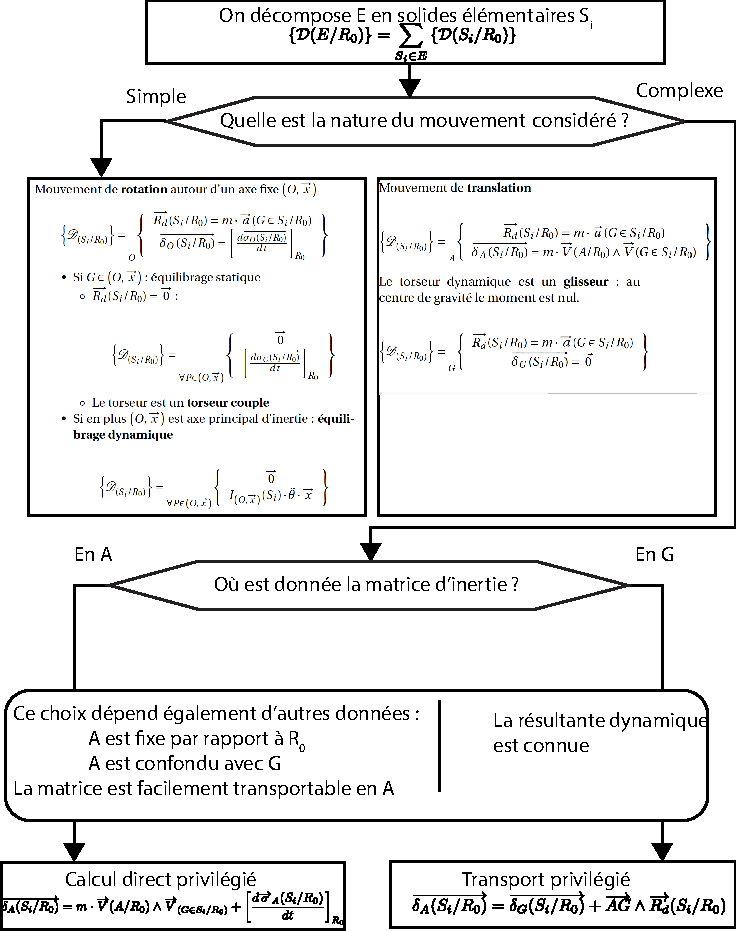
\includegraphics[width=.9\textwidth]{algorigramme_moment_dynamique.pdf}
%\caption{Algorigramme de calcul du moment dynamique \label{algo_moment_dyna}}
\end{center}
%\end{figure}


\begin{thebibliography}{2}
   \bibitem[1]{ref1} Emilien Durif, {\it Cinétique des solides, Lycée La Martinière Monplaisir, Lyon.}
      \bibitem[2]{ref2} Florestan Mathurin, {\it Cinétique, Lycée Bellevue, Toulouse, \url{http://florestan.mathurin.free.fr/}.}
%      \bibitem[3]{ref3} Robert Papanicola, {\it Opérateurs d'inetie, Lycée Charlemagne, Paris, \url{http://sciences-indus-cpge.papanicola.info/}.}
\end{thebibliography}

\newpage

\section*{Bilan}
\footnotesize
\begin{center}
\rotatebox{90}{
\begin{tabular}{|c|c|c|c|}
\hline
Point considéré & Point quelconque $A$ & Centre de gravité $G$  & Point fixe dans $\mathcal{R}_0$ $A$  \\
\hline
&&& \\
Torseur cinétique$\torseurcin{C}{S}{R_0}$
& 
$\torseurl{
\overrightarrow{R_c}(S/R_0)=m\;\overrightarrow{V}(G/R_0)
}{\vectmc{A}{S}{R_0}=\inertie{A}{S}\cdot \vecto{S}{R_0}+m\;\vect{AG}\wedge \vectv{A}{S}{R_0}
}{A}$ 
&
$\torseurl{
\overrightarrow{R_c}(S/R_0)=m\;\overrightarrow{V}(G/R_0)
}{
\vectmc{G}{S}{R_0}=\inertie{G}{S}\cdot \vecto{S}{R_0}
}{G}$
&
$\torseurl{
\overrightarrow{R_c}(S/R_0)=m\;\overrightarrow{V}(G/R_0)
}{
\vectmc{A}{S}{R_0}=\inertie{A}{S}\cdot \vecto{S}{R_0}
}{A}$
\\
&&& \\ \hline
&&& \\
Torseur dynamique $
\torseurcin{D}{S}{R_0}$ & 
$
\torseurl{
\overrightarrow{R_d}(S/R_0)=m\;\overrightarrow{\Gamma}(G/R_0)
}{
\vectmd{A}{S}{R_0}=\left[\frac{\dd \vectmc{A}{S}{R_0}}{\dd t}\right]_{R_0}+\overrightarrow{V(A/R_0)}\wedge \overrightarrow{R_c}(S/R_0)
}{A}
$
&
$
\torseurl{
\overrightarrow{R_d}(S/R_0)=m\;\overrightarrow{\Gamma}(G/R_0)
}{
\vectmd{G}{S}{R_0}=\left[\frac{\dd \vectmc{G}{S}{R_0}}{\dd t}\right]_{R_0}
}{G}
$
&
$
\torseurl{
\overrightarrow{R_d}(S/R_0)=m\;\overrightarrow{\Gamma}(G/R_0)
}{
\vectmd{A}{S}{R_0}=\left[\frac{\dd \vectmc{A}{S}{R_0}}{\dd t}\right]_{R_0}
}{A}
$
\\ 
&&& \\ \hline
\end{tabular}}

\end{center}


\normalsize